% act_d1_login.tex — Iskole: Login & Password Reset
\documentclass[a4paper,landscape]{article}
\usepackage[a4paper,landscape,top=1.8cm,bottom=1.2cm,left=1.2cm,right=1.2cm]{geometry}
\usepackage[dvipsnames,svgnames]{xcolor}
\usepackage{tikz}
\usetikzlibrary{shapes.geometric,arrows.meta,calc}
\usepackage{fancyhdr}
\definecolor{ColHdr} {RGB}{30,58,138}
\definecolor{ActFill}{RGB}{219,234,254}
\definecolor{ActLine}{RGB}{52,109,219}
\definecolor{SysFill}{RGB}{220,254,220}
\definecolor{SysLine}{RGB}{34,139,34}
\definecolor{DecFill}{RGB}{254,244,220}
\definecolor{DecLine}{RGB}{204,120,0}
\definecolor{SwimBg} {RGB}{240,240,248}
\tikzset{
  nd_start/.style={circle,fill=black,minimum size=10pt,inner sep=0pt},
  nd_stop/.style={circle,fill=black,draw=black,double,double distance=2pt,minimum size=10pt,inner sep=0pt},
  nd_act/.style={rectangle,rounded corners=3pt,draw=ActLine,fill=ActFill,text width=4.9cm,minimum height=0.62cm,align=center,font=\footnotesize},
  nd_sys/.style={rectangle,rounded corners=3pt,draw=SysLine,fill=SysFill,text width=4.9cm,minimum height=0.62cm,align=center,font=\footnotesize\itshape},
  nd_dec/.style={diamond,aspect=2.4,draw=DecLine,fill=DecFill,text width=2.5cm,align=center,font=\footnotesize,inner sep=1pt},
  arr/.style={-{Stealth[length=5pt,width=4pt]},thick},
  lbl/.style={font=\scriptsize,fill=white,inner sep=1pt},
}
\pagestyle{fancy}\fancyhf{}
\fancyhead[C]{\bfseries\color{ColHdr}Iskole — Activity Diagram 1: User Login \& Password Reset}
\fancyfoot[C]{\small\thepage}
\renewcommand{\headrulewidth}{1pt}
\renewcommand{\headrule}{\hbox to\headwidth{\color{ColHdr}\leaders\hrule height 1pt\hfill}}
\setlength{\headheight}{16pt}
\begin{document}
\begin{center}
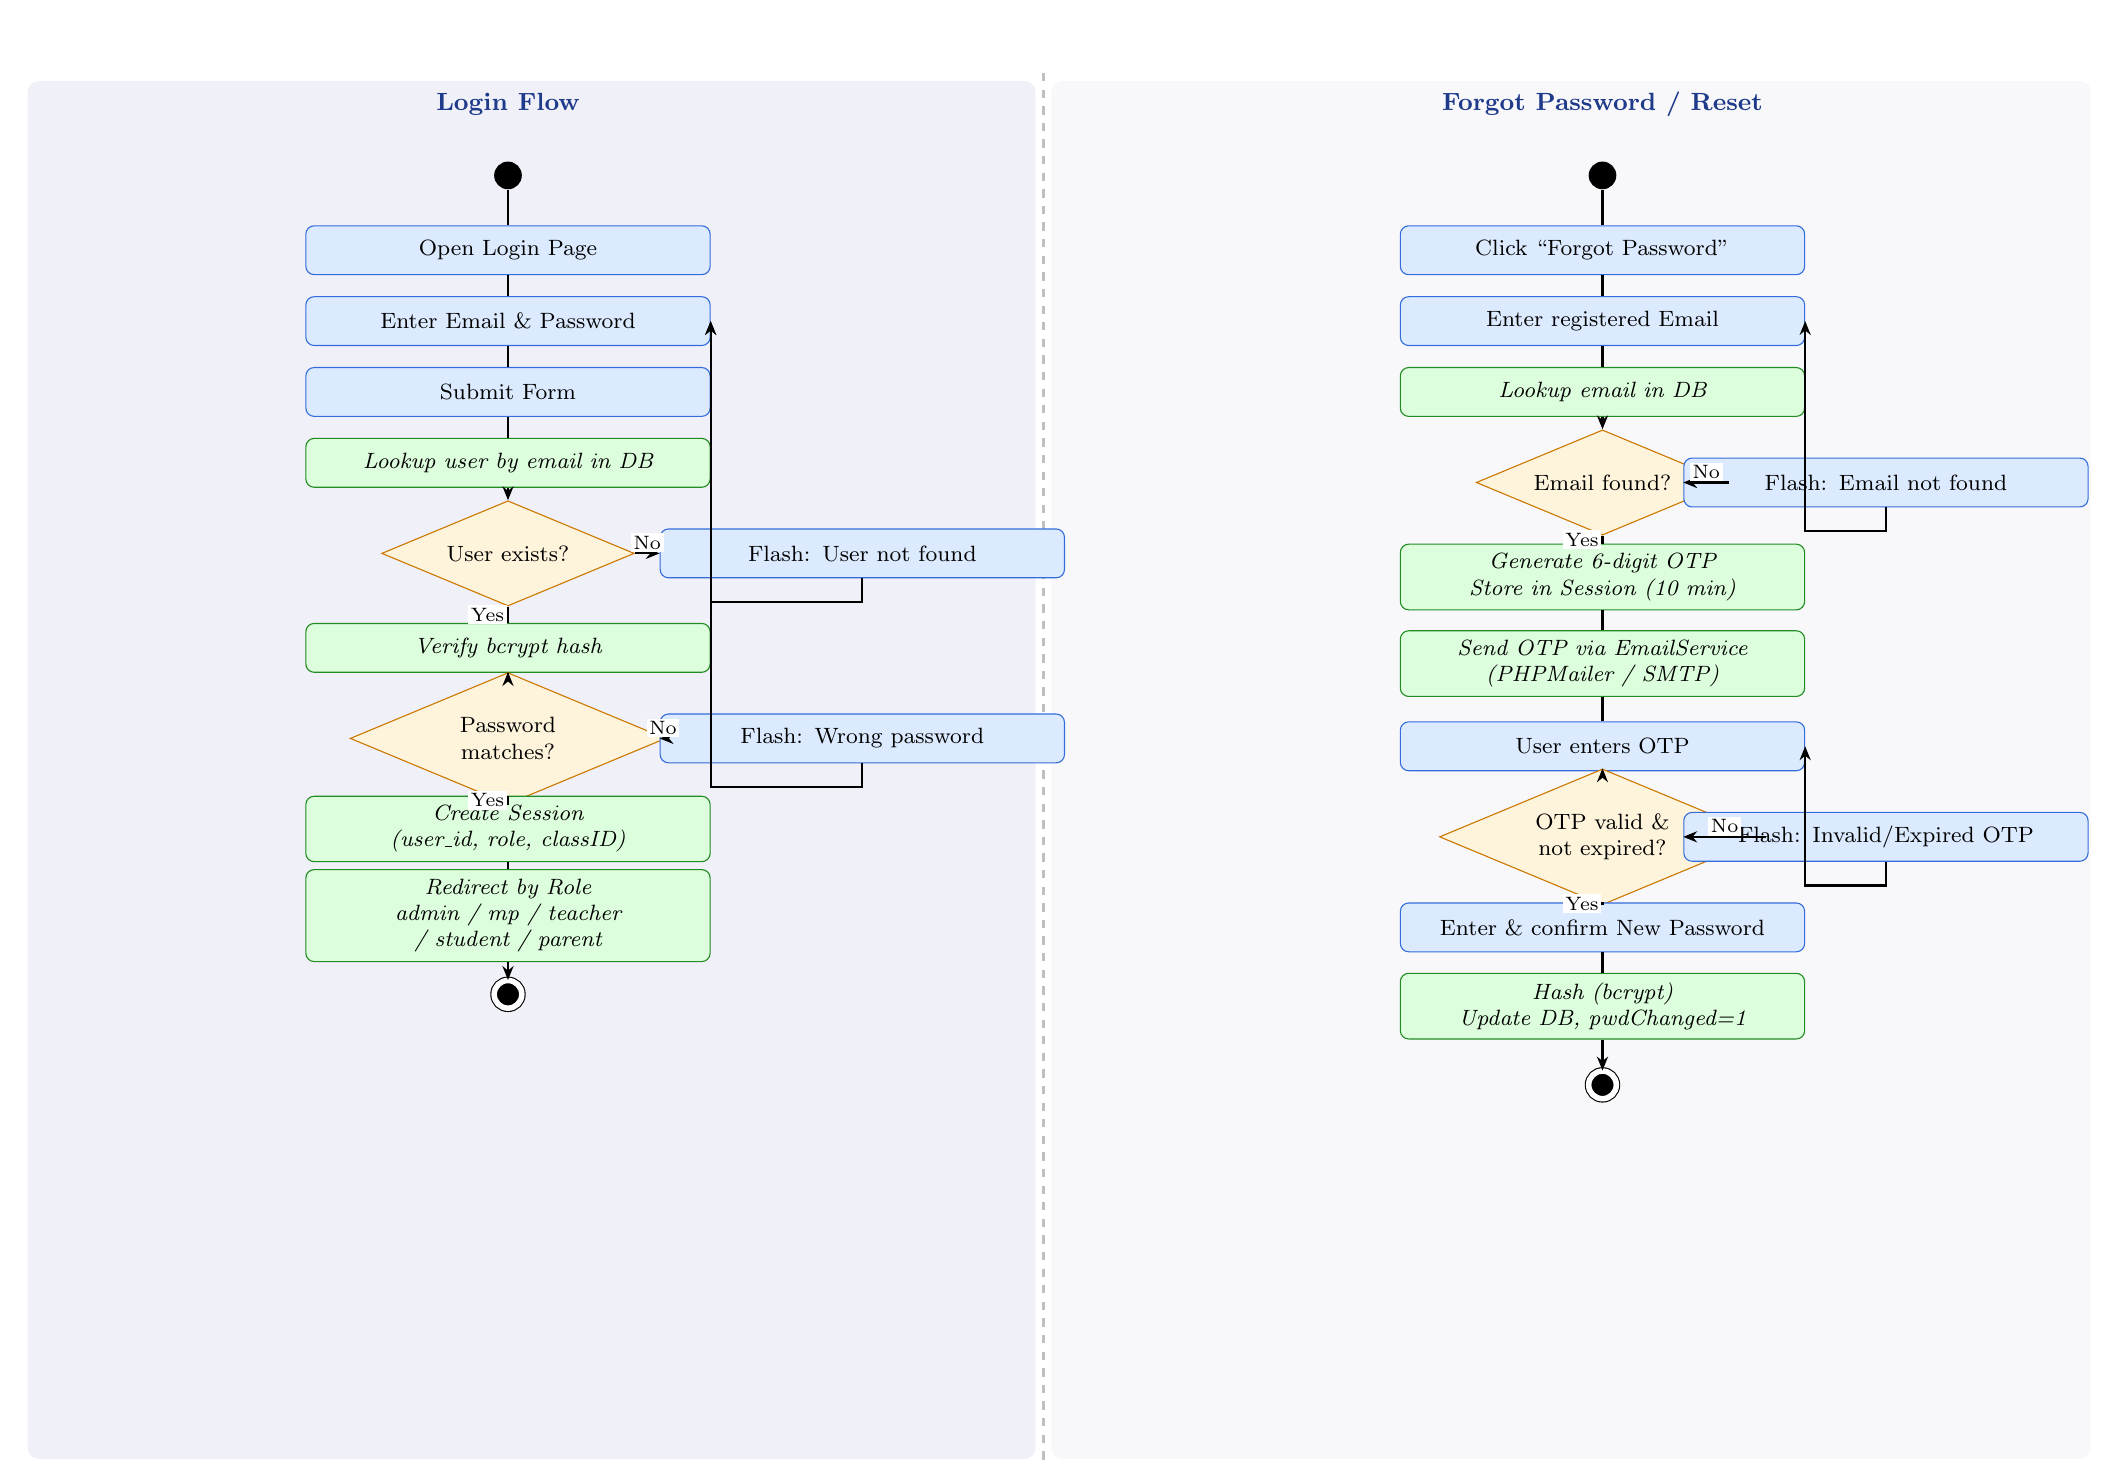
\begin{tikzpicture}[x=1cm,y=1cm]

\def\Lx{6.3}\def\Rx{20.2}

% backgrounds
\fill[SwimBg,rounded corners=4pt](0.2,0.5) rectangle (13,-17);
\fill[SwimBg!50!white,rounded corners=4pt](13.2,0.5) rectangle (26.4,-17);
\node[font=\small\bfseries\color{ColHdr}] at (\Lx,0.2) {Login Flow};
\node[font=\small\bfseries\color{ColHdr}] at (\Rx,0.2) {Forgot Password / Reset};
\draw[dashed,gray!50,thick](13.1,0.6)--(13.1,-17.2);

% LEFT: Login
\node[nd_start] at (\Lx,-0.7) (LS){};
\node[nd_act]   at (\Lx,-1.65)(L1){Open Login Page};
\node[nd_act]   at (\Lx,-2.55)(L2){Enter Email \& Password};
\node[nd_act]   at (\Lx,-3.45)(L3){Submit Form};
\node[nd_sys]   at (\Lx,-4.35)(L4){Lookup user by email in DB};
\node[nd_dec]   at (\Lx,-5.5) (D1){User exists?};
\node[nd_sys]   at (\Lx,-6.7) (L5){Verify bcrypt hash};
\node[nd_dec]   at (\Lx,-7.85)(D2){Password matches?};
\node[nd_sys]   at (\Lx,-9.0) (L6){Create Session\\(user\_id, role, classID)};
\node[nd_sys]   at (\Lx,-10.1)(L7){Redirect by Role\\admin / mp / teacher / student / parent};
\node[nd_stop]  at (\Lx,-11.1)(LE){};
\node[nd_act]   at (\Lx+4.5,-5.5) (E1){Flash: User not found};
\node[nd_act]   at (\Lx+4.5,-7.85)(E2){Flash: Wrong password};

\draw[arr](LS)--(L1)--(L2)--(L3)--(L4)--(D1);
\draw[arr](D1)--node[lbl,left]{Yes}(L5)--(D2);
\draw[arr](D2)--node[lbl,left]{Yes}(L6)--(L7)--(LE);
\draw[arr](D1)--node[lbl,above]{No}(E1);
\draw[arr](D2)--node[lbl,above]{No}(E2);
\draw[arr](E1.south)--($(E1.south)+(0,-0.3)$)-|(L2.east);
\draw[arr](E2.south)--($(E2.south)+(0,-0.3)$)-|(L2.east);

% RIGHT: Forgot Password
\node[nd_start] at (\Rx,-0.7) (RS){};
\node[nd_act]   at (\Rx,-1.65)(R1){Click ``Forgot Password''};
\node[nd_act]   at (\Rx,-2.55)(R2){Enter registered Email};
\node[nd_sys]   at (\Rx,-3.45)(R3){Lookup email in DB};
\node[nd_dec]   at (\Rx,-4.6) (RD1){Email found?};
\node[nd_sys]   at (\Rx,-5.8) (R4){Generate 6-digit OTP\\Store in Session (10 min)};
\node[nd_sys]   at (\Rx,-6.9) (R5){Send OTP via EmailService\\(PHPMailer / SMTP)};
\node[nd_act]   at (\Rx,-7.95)(R6){User enters OTP};
\node[nd_dec]   at (\Rx,-9.1) (RD2){OTP valid \&\\not expired?};
\node[nd_act]   at (\Rx,-10.25)(R7){Enter \& confirm New Password};
\node[nd_sys]   at (\Rx,-11.25)(R8){Hash (bcrypt)\\Update DB, pwdChanged=1};
\node[nd_stop]  at (\Rx,-12.25)(RE){};
\node[nd_act]   at (\Rx+3.6,-4.6) (RE1){Flash: Email not found};
\node[nd_act]   at (\Rx+3.6,-9.1) (RE2){Flash: Invalid/Expired OTP};

\draw[arr](RS)--(R1)--(R2)--(R3)--(RD1);
\draw[arr](RD1)--node[lbl,left]{Yes}(R4)--(R5)--(R6)--(RD2);
\draw[arr](RD2)--node[lbl,left]{Yes}(R7)--(R8)--(RE);
\draw[arr](RD1)--node[lbl,above]{No}(RE1);
\draw[arr](RD2)--node[lbl,above]{No}(RE2);
\draw[arr](RE1.south)--($(RE1.south)+(0,-0.3)$)-|(R2.east);
\draw[arr](RE2.south)--($(RE2.south)+(0,-0.3)$)-|(R6.east);

\end{tikzpicture}
\end{center}
\end{document}
